\documentclass[%
  chapterprefix=false,%
  open=right,%
  twoside=true,%
  paper=a4,%
  logofile={Figures/logo.png},%
  thesistype=master,%
  UKenglish,%
]{se2thesis}
\listfiles
\usepackage[ngerman,main=UKenglish]{babel}
\usepackage{blindtext}
\usepackage[%
  csquotes=true,%
  booktabs=true,%
  siunitx=true,%
  minted=true,%
  selnolig=true,%
  widowcontrol=false,%
  microtype=true,%
  biblatex=true,%
  cleveref=true,%
]{se2packages}

\usepackage{algorithm}
\usepackage{algpseudocode}
\usepackage{multirow}
\usepackage{amsmath}
\usepackage{hyperref}
\usepackage[caption=false]{subfig}

\addbibresource{ref.bib}



\newcommand{\classname}[1]{\texttt{#1}}
\newcommand{\callable}[1]{\texttt{#1}}
\newcommand{\field}[1]{\texttt{#1}}

\author{Gonzalo A. Oberreuter Álvarez}
\title{Effects of the Implementation of a Graph-Based Object Synthesis Heuristic on Pynguin}
\degreeprogramme{Computer Science}
\matrnumber{110082}
\supervisor{Prof.\,Dr.~Gordon Fraser}
\external{Prof.\,Dr.~Christian Hammer}
\advisor{}
\department{Faculty of Mathematics and Informatics}
\institute{Chair of Software Engineering}
\location{Passau}

\begin{document}

\frontmatter

\maketitle

\iffalse{}

\authorshipDeclaration{}

\begin{abstract}
  An English abstract to the thesis. 
  TBD.\@
\end{abstract}

\begin{abstract}[german]
  Eine deutschsprachige Zusammenfassung der Arbeit.
  TBD.\@
\end{abstract}

\begin{acknowledgements}
  Some acknowledgements. 
  TBD.\@
\end{acknowledgements}

\tableofcontents

\fi

\mainmatter{}

\chapter{Introduction}

Software Testing is one of the key aspects of Software Developing while trying to ensure quality over a final product, regardless of the context in which the developing process is made.
This quality can be achieved by the insight provided by the result of the tests, and even because of the defects that can be encountered during the testing phase.
Nonetheless, even though coding different kinds of tests is a good practice, it is often ignored by new or inexpert developers, who also make this mistake halfway by not getting a complete introspection of their own code or, in other words, not getting a complete kind of test coverage.
As of 2017, a study by Trauch and Grabowski~\cite{DBLP:conf/icst/TrautschG17} presented that, over more than 4 million tests, most of them were not correctly categorized (as unit test or not) and approximately half of them use mocking as a testing technique, which tells some aspects about the developing community of the projects in review. 
With this general idea into mind, is that researchers in the last decade   have put effort into autonomous test generation, the concept that implies the usage of different methods or techniques in order to identify patterns and generate test sets with little to zero external intervention.
In 2015, empirical proof was found who showed the following statements about the usage of automated Java unit test generation:
\begin{itemize}
  \item It increases the general structural coverage
  \item It does not lead to the detection of more faults
  \item It affects negatively the ability to capture intended class behaviour
\end{itemize}
according to Fraser et al.~\cite{DBLP:journals/tosem/FraserSMAP15}
The results of this study state fundamentally that this behaviour  comes from the early stages of the tool in question, and proposes to put more work into the readability of generated tests and  the process of test making itself.

Although automatic test generation is achievable with no major problem for statically typed languages like Java~\cite{DBLP:journals/tse/FraserA13} or C, dynamically typed languages such as Python, JavaScript or Lua enforce problems at the time of generating correct arguments for the execution of methods or functions under test.
The major concerns about the argument generation, is that the lack of type information produces ambiguity for the heuristics of the tool at hand at the moment of synthesizing non-primitive types.
Also, the complexity of these class instances in terms of their internal field values might produce runtime errors, which imply a local optima in the search landscape of the test representation~\cite{DBLP:conf/sigsoft/0001O00D21} and therefore an upper bound for coverage.

Within the scope of Python testing, Pynguin~\cite{DBLP:conf/icse/LukasczykF22} is command line interface for the generation of unit tests that applies various algorithms for input generation, such as DynaMOSA~\cite{DBLP:journals/tse/PanichellaKT18}, MIO~\cite{DBLP:conf/ssbse/Arcuri17}, MOSA~\cite{DBLP:conf/icst/PanichellaKT15}, Whole Test Suite~\cite{DBLP:journals/tse/FraserA13}, among others.

At the time of its original release (25th of July 2020), Pynguin was a state-of-the-art open source tool that has been the first step for subsequent researches about how to improve the performance and functionalities of Pynguin itself, including CodaMOSA~\cite{DBLP:conf/icse/LemieuxILS23}, PyLC~\cite{DBLP:conf/sac/SalariEAS23} and many other tools that will be briefly explained in the Section~\ref{chap:related_work}.
These recent new extensions of Pynguin and the latter aforementioned problem at the time of generating complex object inputs are the principal motivations of this thesis and the related and future work to it.

The original Pynguin research paper~\cite{DBLP:conf/icse/LukasczykF22} stated that after the test generation of 118 Python modules, the average branch coverage over all algorithms was $66.8\%$, which leads to think that improvement is possible.

The current Master's thesis proposes an addition to the original structure of Pynguin~(see~Figure~\ref{fig:pyn}), specifically to the \classname{GenerationAlgorithm} abstract class, by developing a Graph-Based Object Synthesis approach~\cite{DBLP:conf/sigsoft/0001O00D21} (GBOS) for the static analysis of Python at bytecode level in order to generate suitable object inputs, diminish the branch coverage gap, and empirically study the effect of the presence of type information in this same generation heuristic.

\begin{figure}
    \inputminted[linenos]{python}{Figures/example.py}
    \caption{Module example.py\label{lst:1}}
\end{figure}

\begin{figure}
  \inputminted[linenos]{python}{Figures/dependencies.py}
  \caption{Dependency module of example.py\label{lst:2}}
\end{figure}

As an example, Listings~\ref{lst:1}~and~\ref{lst:2} represent a MUT and its dependency module, respectively, in which lines 8, 10 and 12 of the MUT are the targets of the branch coverage problem.
Even though the test suite generated by Pynguin (see Listing~\ref{lst:3}) gets to a branch coverage of \(37.5\%\) (using DynaMOSA, the seed 1998 and 100 seconds as stopping condition), it can be inferred that this result comes from \verb|test_case_1()|, that executes one of the first two branches in the MUT and checks if the variables \verb|actor| and \verb|target| are actual \verb|Player| objects.
This behaviour prevents Pynguin from escaping a local optima for the branch coverage of line 12.
At this point, the idea of using a graph for the synthesis of objects is to get Pynguin to generate a \verb|GameState| object with the necessary \verb|Players| in the \verb|players| list, and a \verb|Action| object with correct attributes, so a hypothetical test could reach the third branch in the MUT, even if it is with a false guard.
  
\begin{figure}
    \inputminted[linenos]{python}{Figures/test1.py}
    \caption{Test suite generated by Pynguin for module example.py\label{lst:3}}
\end{figure}

The Graph-Based heuristic proposed by Lin et al.~\cite{DBLP:conf/sigsoft/0001O00D21} generates an Object Construction Graph (OCG) from a previous code slicing, performed from the program dependency graph and a specific target branch as criteria.
This branch must be selected from those who have not reached their full coverage, or are ``non-trivial'', and the depth of the intra procedural dependency should be set as an arbitrary level $t_{\text{dep}}$.
Then, this OCG is used to generate a code template that should be directly into the test code representation of Pynguin, for it to be then evolved or modified by one of the available Search-Based algorithms.
Pynguin, similarly to other Search-Based test generating tools, represents its test cases as a sequence of implementations of a super class \classname{Statement} that can be later transformed into an Abstract Syntax Tree (AST) and an actual block of Python code.
This previous idea was completely implemented in and for Java, which means that part of the work to be done is to ideate a new Python representations of the OCG.\@
Listing~\ref{lst:4} shows the code of a statement sequence template for the testing of the example module that still gets a run time error in line 18.
However, this template allows Pynguin to get out of the local optima, if right values are modified in the correct variables.

\begin{figure}
  \inputminted[linenos]{python}{Figures/template.py}
  \caption{Potential test template obtained through the use of an OCG\label{lst:4}}
\end{figure}

A type information gathering mechanism (e.g.~the analysis of every method or function AST) will be applied in order to review the modules in the testing set of the experimental setup and how the general type information of a Python module affects in the ability of the GBOS approach to generate correct object inputs templates.
The reason for this is, as stated before, Python being a dynamically typed language and not requiring the type of variables in the script in order to be executed.
To illustrate this, if line 4 in Listing~\ref{lst:1} were to be replaced to \mint{python}|def checkRules(self, action, state) -> bool:| it would make Pynguin not have any information about the type of the parameters, and generate a test suite similar to the one in Listing\ref{lst:5}.
The behaviour that allows Pynguin to generate the previous suite imply that the current type system implemented as part of Pynguin does not work properly when trying to infer object types.

\begin{figure}
  \inputminted[linenos]{python}{Figures/test2.py}
  \caption{Test suite generated by Pynguin for a variation of module example.py\label{lst:5}}
\end{figure}

After the implementation part is done, a study of the extension will be made through the selection of arbitrary sets of Python modules, being these either the original research paper's or a new super set that ensures the explicit type of object inputs and a ratio of this kind of inputs that surpasses $50\%$.
The final purpose of the thesis is to obtain a Cohen's d effect size over the coverage results between Pynguin and the proposed extension, and compare it to the ones obtained between EvoSuite and EvoObj.
A further analysis of the difference in this metric shall also be done.

The previous setup can be structured by the following research questions and further explained by their experimental implications:

\resq{Can the Graph-Based Object Synthesis extension outperform Pynguin in its original paper's experimental setup similarly as EvoObj did with EvoSuite?}

For the answer of this Research Question, the archive of the projects used for the experimental setup of Pynguin in its release paper\footnote{https://zenodo.org/records/6838658} will be put again to the test to benchmark the performances of both Pynguin in its latest version (0.25.0) and the extension to the tool to be presented by this thesis.
While trying to follow a similar configuration to the one presented in all the papers featuring Pynguin, all the algorithms available in the latest version will be executed with their default settings, and 30 times per module.

\resq{Is there a correlation between the difference in coverage results and the amount of object-like callable inputs of MUTs while using Pynguin and the GBOS extension?}

In this scenario, the same module archive from the previous research question will be used, but trivial modules with coverages that go \(100\%\) in a short amount of time (e.g. 10 seconds) will be filtered.
Then, default parameters of the available algorithms and 30 runs per module will be executed, in order to obtain the coverage results of both versions of Pynguin and calculate a coverage delta per module.
Finally, the percentage of object-like inputs in methods will be obtained by analysing the AST of the MUTs with the following formula
\[ \frac{1}{n}\sum_{m_i \in M} \frac{o_i}{p_i}\]
where \(M\) is a MUT, \(m_i\) a method, \(p_i\) the amount of parameters in \(m_i\), \(o_i\) the amount of object-like parameters in \(m_i\), and \(n\) the amount of methods in \(M\). 


\chapter{Background}

\section{Pynguin}

The \textbf{PY}tho\textbf{N} \textbf{G}eneral \textbf{U}n\textbf{I}t test ge\textbf{N}erator (Pynguin) is a Command Line Interface software intended for the automatic generation of unit tests for Python modules.
Its way of generating these Unit tests, is by using a different selection of search-based algorithms oriented to the test generation task, taken straightforward from the literature and implemented according to the internal representation in an Object-Oriented paradigm.
% TODO - Mention the assertion generation
Throughout the years after its release, Pynguin has had many updates\footnote{https://www.pynguin.eu/blog/} that have improved its test generation performance and outputs, from which are notable: the addition of line and checked coverage~\cite{DBLP:conf/icst/SchulerZ11}, to the default branch coverage; the implementation of a native type system and the integration with Type4Py~\cite{DBLP:conf/icse/MirLPG22} for their usage in the correct type setting while generating variable statements; and the extended analysis of mutation's effects on tests for the correct generation of assertions.

As mentioned before, the main core of Pynguin's test representation is the abstract class \classname{Statement}, and its subsequent wrapper classes \classname{TestCase}, containing a list of \classname{Statement} instances, and \classname{TestCaseChromosome}, containing a \classname{TestCase}.
In the prior one, the next child classes available are \classname{AssignmentStatement}, a direct assignment of any kind of reference to a variable (e.g.~foo.bar = var\_1); and \classname{VariableCreatingStatement}, representing anything that can be assigned to a variable such as primitive types, collection types, fields, or any type of call (e.g.~int\_1~=~1, list\_1~=~list\(()\), foo~=~Foo\((\text{int\_1,~list\_1})\)).
The following hierarchy of these two can be represented by Figure~\ref{fig:hierarchy}.

\begin{figure}[h]\label{fig:hierarchy}
  \centering
  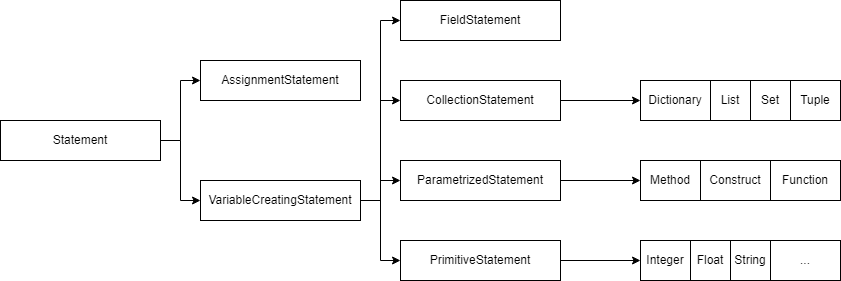
\includegraphics[width=1\textwidth]{Figures/statement_hierarchy2.png}
  \vspace*{0.5cm}
  \caption{Hierarchy of the \classname{Statement} class.}
\end{figure}

One class that assures Pynguin's easiness at the time of expanding it, is the abstract class \classname{GenerationAlgorithm}, which works as a layout for the insertion of any new heuristic of algorithm into the tool's current options, for the generation of \classname{TestSuiteChromosome}, another class wrapper for a list of \classname{TestCaseChromosome}.

In the context of evolutionary and genetic algorithms, the \classname{Statement} class has an abstract method called \(\text{\callable{mutate}}()\), which depending on the instance's final class, mutates either the primitive value, or the references that are encapsulated in it.

About the available algorithms, Pynguin has a total of 7 available: Random, Random Test Case Search, Random Test Suite Search, Whole Suite, MIO, MOSA and DynaMOSA.\@
From these, the experimental phase will be done mostly considering the last 4, because those implement either an archive or a dynamic chromosome population, which is necessary for the extension.

\begin{figure}[tb]
  \centering
  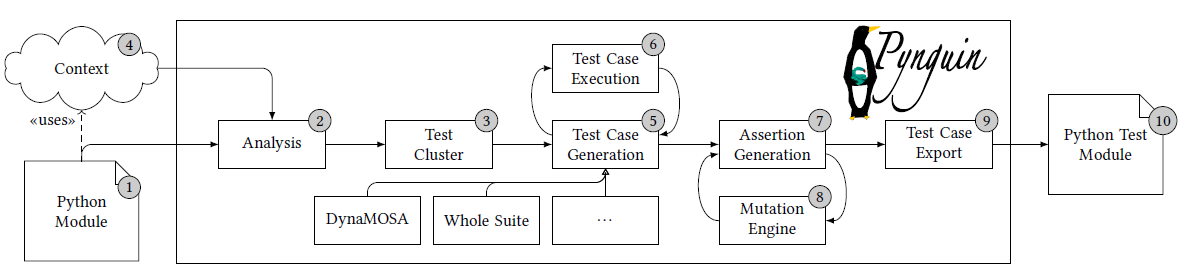
\includegraphics[width=.99\textwidth]{Figures/pynguin.png}
  \caption{Pynguin structure}\label{fig:pyn}
\end{figure}

Pynguin's workflow structure is presented in Figure~\ref{fig:pyn} and consists of 10 steps that work in the following manner
\begin{enumerate}
  \item The unit test generation process starts with the input of a user defined python module that needs to be tested.
  \item The module is then analysed in order to obtain primordial information, such as all the functions, classes and their respective attributes and methods, together with their respective parameters.
  \item In the Test Cluster, all relevant information is gathered from the analysis of the module under test (MUT) and its dependencies.
  \item As mentioned in the previous item, the Context step performs an inter procedural analysis of all the libraries and modules used by the actual MUT, and joins any new obtained information with the data in the Test Cluster.
  \item The Test Case Generation step, individually picks functions or methods from the Test Cluster in order to generate instances of the \classname{Statement} class, firstly by generating a certain amount of either primitive, collection or instance statement used as parameter arguments, and then by generating the respective callable, owner of the different branches or lines to cover.
  \item After a Test Case Generation is performed, it is executed to get the desired coverage and analyse if (a) it already reached a full coverage or (b) a new better Test Case should be generated.
  \item Once the stopping conditions are met, the test cases are finished with an optional assertion to check the results of the test.
  \item Alternatively, mutations of the test cases are created using MutPY, so Pynguin can evaluate if the previously created assertion kill or not the mutants.
  If they do not, new assertions are created.
  \item In the Export step, Pynguin transforms the test cases from their chromosome representation into a Python AST representation and then into a Python test with the correspondent decorators of the library PyTest.
  \item Finally, these tests are written into a final module.
  
\end{enumerate}


\section{MOSA}

The Many-Objective Sorting Algorithm~\cite{DBLP:conf/icst/PanichellaKT15} (MOSA), is an improvement to the classic Multi-objective Optimization algorithms (MOA) such as the Non-dominated Sorting Genetic Algorithm II (NSGA-II) or the Strength Pareto Evolutionary Algorithm (SPEA2), and applied taking into account some specific draw backs of the branch coverage problem in test generation, such as the great computational effort needed by these classic algorithms when working with a number of objectives bigger than an order of magnitude of 10.
In the same direction, another challenge that MOSA was able to overcome, is the selection and persistence over a non-dominated sort of those tests that have the best branch distance regarding non-covered goals.

Algorithm~\ref{alg:MOSApseudo} shows an overview of MOSA's pseudocode, which follows a similar structure compared to NSGA-II's behaviour.
Both start with the generation of an initial random population, but the presence of a test archive to store the current best solutions per target is the first difference (lines 1 and 3).
Then, in every iteration an offspring is computed by means of arbitrary selection, crossover and mutation methods, which later is sorted into Pareto frontiers using the Preference Sorting (line 13).
This procedure is the one mentioned before, which at the beginning sets into the first frontier the best tests according to a preference criterion (usually the desired coverage), and then realizes a common Fast Non-dominated Sort over the rest of tests.
Finally, MOSA finishes every iteration of itself filling the next population with the right amount of tests from all the available Pareto frontiers, with the slight difference from NSGA-II that MOSA uses a sub-vector dominance assignment~\cite{DBLP:conf/issta/KifetewPLOT13} for the Crowding Distance Assignment (line 12).

About the MOSA implementation in Pynguin, it follows the same structure as the one in Algorithm~\ref{alg:MOSApseudo}.


\algrenewcommand\algorithmicrequire{\textbf{Input}}
\algrenewcommand\algorithmicensure{\textbf{Output}}


\begin{algorithm}[htb]
  \centering
  \caption{MOSA Pseudocode}\label{alg:MOSApseudo}
  \begin{algorithmic}[1]
    \Require~Stopping condition \(C\), Set of program targets \(B\), Population size \(M\)
    \Ensure~A test suite \(T\)
    \State~\(A \gets \{\}\)
    \State~\(P_t \gets \text{GenerateRandomPopulation}()\)
    \State~\(\text{UpdateArchive}(A, P_t)\)
    \While{\(\neg C\)}
      \State~\(Q_t \gets \text{GenerateOffspring}(P_t)\)
      \State~\(\text{UpdateArchive}(A, P_{t+1})\)
      \State~\(R_t \gets P_t \cup Q_t\)
      \State~\(F_x \gets \text{PreferenceSorting}(R_t)\)
      \State~\(P_{t+1} \gets \emptyset \)
      \State~\(d \gets 0\)
      \While{\(|P_{t+1}| + |F_d| \leq M\)}
        \State~\(\text{CrowdingDistanceAssignment}(F_d)\)
        \State~\(P_{t+1} \gets P_{t+1} \cup F_d\)
        \State~\(d \gets d + 1\)
      \EndWhile\@
      \State~\(\text{CrowdingDistanceSort}(F_d)\)
      \State~\(P_{t+1} \gets P_{t+1} \cup F_d[1\: (M - |P_{t+1}|)]\)
    \EndWhile\@
  \end{algorithmic}
\end{algorithm}

\section{DynaMOSA}\label{sec:dynamosa}

DynaMOSA comes as a further extension of MOSA by Panichella et al.~\cite{DBLP:journals/tse/PanichellaKT18}, with the addition of a dynamic selection of the targets to be included into the first Pareto Frontier when executing the preference sorting.
The idea of including a dynamic selection of targets starts from the representation of a program into a Control Flow Graph \(\text{CFG} = \langle V_{\text{CFG}}, E_{\text{CFG}} \rangle\) where every node represents an abstraction of statements or basic blocks and every directed edge, a path of execution.
With the CFG, it is possible to realize how those uncovered targets that have one or more already reached target predecessor are redundant to try to cover because they will always have objective score of \(f_r = \text{BranchDistance}(b) + 1\), where (\(+1\)) represents the approach level or the distance in the CFG to reach the successive target.
This means that every target can be prioritized into a hierarchy according to the definition of a Control Dependency Graph (CDG).

Before defining the elements of a CDG, it is necessary to define the concepts
%plagio?
\begin{itemize}
  \item \textbf{Dominator}: a statement \(v_1\) dominates another statement \(v_2\), if every execution path to \(v_2\) in the CFG goes through \(v_1\).
  \item \textbf{Post-Dominator}: a statement \(v_1\) post-dominates another statement \(v_2\), if every execution path from \(v_2\) to an exit node in the CFG goes through \(v_1\).
\end{itemize}
Then, a \(\text{CDG} = \langle V_{\text{CDG}}, E_{\text{CDG}} \rangle\) is a graph where \(V_{\text{CDG}} = V_{\text{CFG}}\), and for every pair \(v_1, v_2 \in V_{\text{CDG}}\), there is a directed edge \((v_1, v_2)\) if and only if \(v_2\) is not a post-dominator of \(v_1\) and there is a path in the \(CFG\) between \(v_1\) and \(v_2\) whose nodes are not post-dominated by \(v_2\).
This edge represents a control dependency between both statement blocks.

The pseudocode of DynaMOSA is shown in Algorithm~\ref{alg:DynaMOSApseudo}, with the only differences to MOSA being found in the lines 1, 5 and 9 when calling the set of an initial set of non-dependant targets and the dynamic update of these.
The \(\text{UpdateTarget}()\) procedure, is applied inside Pynguin by implementing a class for, a Control Flow Graph (named \classname{CFG}), as a wrapper of the \classname{ControlFlowGraph} class from the Python \classname{bytecode} module; and a Control Dependency Graph (called \classname{ControlDependenceGraph}).
Both of these classes are a fundamental part for the proposed heuristic implementation.

% TODO - anything else to fill?

\begin{algorithm}[htb]
  \centering
  \caption{DynaMOSA Pseudocode}\label{alg:DynaMOSApseudo}
  \begin{algorithmic}[1]
    \Require~Stopping condition \(C\), Set of program targets \(B\), Population size \(M\), Control dependency graph \(G\), \(\phi\)~Map between edges of \(G\) and targets
    \Ensure~A test suite \(T\)
    \State~\(U^* \gets \text{NonDependentTargets}(B)\)
    \State~\(A \gets \{\}\)
    \State~\(P_t \gets \text{GenerateRandomPopulation}()\)
    \State~\(\text{UpdateArchive}(A, P_t)\)
    \State~\(\text{UpdateTargets}(U^*, G, \phi)\)
    \While{\(\neg C\)}
      \State~\(Q_t \gets \text{GenerateOffspring}(P_t)\)
      \State~\(\text{UpdateArchive}(A, P_{t+1})\)
      \State~\(\text{UpdateTargets}(U^*, G, \phi)\)
      \State~\(R_t \gets P_t \cup Q_t\)
      \State~\(F_x \gets \text{PreferenceSorting}(R_t)\)
      \State~\(P_{t+1} \gets \emptyset \)
      \State~\(d \gets 0\)
      \While{\(|P_{t+1}| + |F_d| \leq M\)}
        \State~\(\text{CrowdingDistanceAssignment}(F_d)\)
        \State~\(P_{t+1} \gets P_{t+1} \cup F_d\)
        \State~\(d \gets d + 1\)
      \EndWhile\@
      \State~\(\text{CrowdingDistanceSort}(F_d)\)
      \State~\(P_{t+1} \gets P_{t+1} \cup F_d[1\: (M - |P_{t+1}|)]\)
    \EndWhile\@
  \end{algorithmic}
\end{algorithm}

\section{Whole Test Suite}

The Whole Test Suite generation algorithm is an instance of a genetic algorithm that, as a result of custom operators, tries to optimize the computational effort of target coverage by evolving a population of test suites in a higher level of abstraction, compared to the other reviewed algorithms so far.
One of the main problems at the time of approaching test generation as a set of individual goals, is the case of encountering unreachable guards due to their recognition being an undecidable problem, and therefore it is not possible for the algorithm at hand to filter these elements in a trivial way.
Following the same though, this algorithm introduces extra upper bounds to the maximum size of a population, for both the amount of test cases that are encapsulated in a test suite (\(N\)) and the amount of statements that a test case can contain (\(L\)), in order to avoid the size of these abstractions to tend to infinite.

Besides the preferred code coverage as fitness function, which is evaluated by running all test cases in a test suite and adding up all covered targets and distances, a secondary fitness function used is the size of the test suite, specifically for the forwarding of offspring chromosomes to further generations.
Algorithm~\ref{alg:WTSpseudo} shows Whole Test Suite's pseudocode, having particular variations from a default genetic algorithm in lines 7, 11, and 12 to 27.
Line 7 holds the crossover operator, that chooses a random value \(\alpha \in [0.0, 1.0]\) and generates 2 test suite offspring from the selected parents by splitting them both at position \(\alpha \times \text{Length}(p)\) and interchanging the segments.
Line 11 locates the mutation operator, where the algorithm mutates both test suites and test cases with a probability inverse to their own size, meaning that statistically only one of each are mutated in every iteration.
For test suites, with probability \(\sigma\) a new test case is added iteratively until the mutation fails.
Concurrently for test cases, three mutations can be applied with probability \(\frac{1}{3}\) each
\begin{itemize}
  \item Remove: every statement of the test case of length \(l\) has a probability \(\frac{1}{l}\) of being deleted from it. For any removed statement, future references to any linked variable are either replaced with another variable with the same data type or deleted recursively.
  \item Change: every statement of the test case of length \(l\) has a probability \(\frac{1}{l}\) of being changed, meaning that it will either generate a new primitive value, add new array elements or call another method/function accordingly.
  \item Insert: a new statement is added into the test case with probability \(\sigma~'\) sequentially until failed, similar to the test suite mutation.
\end{itemize}
The final novelty from this algorithm between lines 12 and 27, is the mechanism of generational forwarding already mentioned, which basically intends to bring the offspring to the next iteration's population only if either it has better fitness value, or if the fitness is equal to the one from the parents and the size of the offspring is much smaller.

In terms of the Whole Test Suite generation algorithm's implementation in Pynguin, it was done by setting a field in the \classname{WholeSuiteAlgorithm} class called \field{\_population}, containing a list of \classname{TestSuiteChromosome} objects.


\begin{algorithm}[htb]
  \centering
  \caption{Whole Test Suite Pseudocode}\label{alg:WTSpseudo}
  \begin{algorithmic}[1]
    \Require~Stopping condition \(C\), Crossover probability \(P_c\)
    \Ensure~A test suite \(T\)
    \State~\(S \gets \text{GenerateRandomPopulation}()\)
    \While{\(\neg C\)}
      \State~\(Z \gets \text{Elitism}(S)\)
      \While{\(|Z| \neq |S|\)}
        \State~\(p_1,\, p_2 \gets \text{ParentRankSelection}(S)\)
        \If{\(P_c > \text{RandomFloat}()\)}
          \State~\(o_1,\, o_2 \gets \text{Crossover}(p_1,\, p_2)\)
        \Else\@
          \State~\(o_1,\, o_2 \gets p_1,\, p_2\)
        \EndIf\@
        \State~\(\text{Mutate}(o_1,\, o_2)\)
        \State~\(f_p \gets \text{MinimumFitness}(p_1,\, p_2)\)
        \State~\(f_o \gets \text{MinimumFitness}(o_1,\, o_2)\)
        \State~\(l_p \gets \text{Length}(p_1) + \text{Length}(p_2)\)
        \State~\(l_0 \gets \text{Length}(o_1) + \text{Length}(o_2)\)
        \State~\(T \gets \text{BestIndividual}(S)\)
        \If{\(f_o < f_p \lor (f_o = f_p \land l_o \leq l_p)\)}
          \For{\(o \in {o_1, o_2}\)}
            \If{\(\text{Length}(o) \leq 2\times \text{Length}(T)\)}
              \State~\(Z \gets Z \cup {o}\)
            \Else\@
              \State~\(Z \gets Z \cup {p_1 \text{or} p_2}\)
            \EndIf\@
          \EndFor\@
        \Else\@
          \State~\(Z \gets Z \cup {p_1, p_2}\)
        \EndIf\@
      \EndWhile\@
      \State~\(S \gets Z\)
    \EndWhile\@
  \end{algorithmic}
\end{algorithm}

\section{MIO}

The Many Independent Objective (MIO) algorithm~\cite{DBLP:journals/infsof/Arcuri18} consists of a modification of the default (1 + 1) evolutionary algorithm, whose author came up with by either taking the most notable characteristics of both MOSA and Whole Test Suite or trying to avoid their limitations, in terms of exploration and exploitation of the search landscape.

One of these limitations, is the presence of a fixed size population that may not be big enough depending on the size of the System Under Test (SUT), the number of objectives to cover, or would not work optimally if too many redundant test have been introduced into it.
To fix this, MIO maintains an archive of test populations per target and sets a maximum amount of tests to be introduced to it.

MIO's core behaviour is represented by the existence of 3 main parameters; \(n\), being the number of tests per target to be stored in the archive; \(P_r\), the probability of introducing a randomly generated test into the population; and \(m\), the maximum amount of mutations to be applied.
To these, the algorithm also adds a fourth parameter \(F\), whose main purpose is to split the stopping conditions' budget in order to have two main phases with different sets of \(n\), \(P_r\) and \(m\).
Within the three parameters, it is stated that the first two are the more relatives ones at the time of controlling the exploration/exploitation.
A summary of all parameters, their respective domain range and their default value implemented in Pynguin is shown in Table~\ref{tab:MIOparams}

A pseudocode of MIO is presented in Algorithm~\ref{alg:MIOpseudo}, which starts by initializing the archive with empty populations.
The following evolution of this population, is firstly made with the selection of either a new random test or one sample from the archive, that is obtained from one of the uncovered goals' populations.
If this sample is from the archive, it is mutated.
Then, for each one of this test's relevant targets \(k\), the test is either added to the archive as a solution in case the goal was covered, or added to its respective population \(T_k\).
Finally, the parameters are updated at the end of the iteration.

With respect to this approach, Pynguin only differs from the original algorithm's idea in the integrations of both \(T\) and \(A\) into a single data structure.

\begin{table}[htb]
  \caption{Search space of MIO's parameters.\label{tab:MIOparams}}
  \centering
  \begin{tabular}{llllc}
  \toprule
  \multicolumn{2}{l}{\textbf{Parameter}}                                                                                        & \textbf{ID} & \textbf{Range}       & \textbf{Default Value} \\ \midrule
  \multicolumn{2}{l}{F-parameter}                                                                                               & \(F\)       & \([0.0,1.0]\)        & \(0.5\)                \\ \cmidrule(lr){1-5}
  \multicolumn{1}{l}{\multirow{3}{*}{Initial Phase}} & Tests per target                                                          & \(n_i\)    & \([1,\infty ]\)      &  \(10\)                \\ \cmidrule(lr){2-5} 
  \multicolumn{1}{l}{}                               & \begin{tabular}[c]{@{}l@{}}Probability to select a \\ random test\end{tabular} & \(P_{ri}\)    & \([0.0,1.0]\)& \(0.5\)                \\ \cmidrule(lr){2-5} 
  \multicolumn{1}{l}{}                               & Number of mutations                                                      & \(m_i\)     & \([1,\infty ]\)      & \(1\)                  \\ \cmidrule(lr){1-5}
  \multicolumn{1}{l}{\multirow{3}{*}{Focused Phase}} & Tests per target                                                          & \(n_f\)    & \([1,\infty ]\)      & \(1\)                  \\ \cmidrule(lr){2-5} 
  \multicolumn{1}{l}{}                               & \begin{tabular}[c]{@{}l@{}}Probability to select a \\ random test\end{tabular} & \(P_{rf}\)    & \([0.0,1.0]\)& \(0.0\)                \\ \cmidrule(lr){2-5} 
  \multicolumn{1}{l}{}                               & Number of mutations                                                      & \(m_f\)     & \([1,\infty ]\)      & \(10\)                 \\ \bottomrule
  \end{tabular}
  \end{table}


\algrenewcommand\algorithmicrequire{\textbf{Input}}
\algrenewcommand\algorithmicensure{\textbf{Output}}


\begin{algorithm}[htb]
  \centering
  \caption{MIO Pseudocode}\label{alg:MIOpseudo}
  \begin{algorithmic}[1]
    \Require~Stopping condition \(C\), Fitness function \(\delta\), Population size limit \(n\), Start~of~focused search \(F\)
    \Ensure~Archive of optimized individuals A
    \State~\(T \gets \text{SetOfEmptyPopulations}()\) 
    \State~\(A \gets \{\}\)
    \While{\(\neg C\)}
      \If{\(P_r > \text{RandomFloat}() \text{or IsEmpty}(T)\)}
        \State~\(p \gets \text{RandomIndividual}()\)
      \Else\@
        \State~\(p \gets \text{SampleIndividual}(T)\)
        \State~\(p \gets \text{Mutate}(p)\)
      \EndIf\@
      \ForAll{\(k \in \text{ReachedTargets}(p)\)}
        \If{\(\text{IsTargetCovered}(k)\)}
          \State~\(\text{UpdateArchive}(A, p)\)
          \State~\(T \gets T \setminus \{T_k\}\)
        \Else\@
          \State~\(T_k \gets T_k \cup \{p\}\)
          \If{\(|T_k| > n\)}
          \State~\(\text{RemoveWorstTest}(T_k, \delta)\)
          \EndIf\@
        \EndIf\@
      \EndFor\@
      \State~\(\text{UpdateParameters}(F, P_r, n, m)\)
    \EndWhile\@
  \end{algorithmic}
  \end{algorithm}


\section{GBOS Heuristic}

% TODO
The Graph Based Object Synthesis heuristic is the name given to the methodology presented by Yun et al.~\cite{DBLP:conf/sigsoft/0001O00D21} for the generation of complex object instances to be used as arguments in methods to be tested in a test case of the Java programming language.
One of the motivations for this research study was the possible non-continuity of test cases' search space with respect to coverage, when some related targets have the need to evaluate multiple conditions on an object instances before even getting an actual distance to them.
% TODO - maybe reference the example in the introduction?
The procedure done by this heuristic, consists of two main phases; the creation of an Object Construction Graph (OCG), that represents all relevant dependency flows of a method from its inputs to the actual target to be reached; and the translation of the OCG into an actual test case template, that serves as an initial search point for the test generation algorithm.

\subsection{OCG generation}

For the generation of the OCG, one must start with the generation of the Program Dependency Graph (PDG), a complete representation of all control and data dependencies of a program.
As stated in Section~\ref{sec:dynamosa}, the control dependencies of a program are represented with the aforementioned CDG.\@
Similarly, the data dependencies of a program can be represented with a Data Dependency Graph \(\text{DDG} = \langle V_{\text{DDG}}, E_{\text{DDG}} \rangle\), where \(V_{\text{DDG}} = V_{\text{CFG}}\) and for every pair \(v_1, v_2 \in V_{\text{DDG}}\), there is a directed edge \((v_1, v_2)\) if and only if there is a variable \(X_{v_1}\) defined in \(v_1\) and used in \(v_2\), that is part of the reaching definitions of \(v_2\).

Reaching definitions~\cite{DBLP:books/aw/AhoSU86} is a data-flow schema in the form of a fixed point algorithm for the recognition of any variable definitions that always reach in or out of a basic block in a program.
For a node \(n \in V_{\text{CFG}}\), representing a basic block in the CFG, \callable{Defines}\((n)\) being the set of variables \(x_n\) defined in \(n\) and \callable{Pre}\((n)\) the predecessor nodes, the following equations set the reaching definitions of node \(n\)

\begin{align*}
  \text{\textbf{gen}}(n) &:= \text{\callable{Defines}}(n) \\
  \text{\textbf{kill}}(n) &:= \bigcup_{v \in V_{\text{CFG}}} x_v, \forall x \in \text{\callable{Defines}}(n) \\
  \text{\textbf{ReachIN}}(n) &:= \bigcup_{p \in \text{\callable{Pre}}(n)} \text{\textbf{ReachOUT}}(p) \\
  \text{\textbf{ReachOUT}}(n) &:= \text{\textbf{gen}}(n) \cup (\text{\textbf{ReachIN}}(n) \setminus \text{\textbf{kill}}(n))\\
\end{align*}

Having the two necessary representations of both a CDG and a DDG, a formal outline of a PDG is the tuple \(\langle V_{\text{PDG}}, E_{\text{PDG}} \rangle\), with \(\langle V_{\text{PDG}} = \langle V_{\text{CFG}}\) and \(E_{\text{PDG}} = E_{\text{CDG}} \cup E_{\text{DDG}}\).

The necessary PDG for the OCG's building process must also be inter-procedural until a certain level of deepness, considering that one or many of the target method's input objects may be modified by a subsequent call.
This new requirement is met by just adding to the main PDG new edges from the correspondent callee's basic block to the entry node of the other method or function PDG, which also needs to be generated beforehand.

After having the full inter-procedural PDG, a node containing a branch \(b\) (chosen target for the heuristic) must be used as entry criteria to apply a backward slice and either

\begin{itemize}
  \item a node with an instruction reading a method input
  \item a node with an instruction reading a global variable
  \item an entry node 
\end{itemize}

as stopping criteria.

The following step, is to analyse the sliced graph and link directly every instance of a node loading the complex method parameter objects with any node from the inter-procedural methods' PDGs that retrieve a field or access an array, so the relevant variable state of these objects can be recorded flawlessly throughout the graph.

Finally, the sliced PDG is sliced further in a forward manner, using the object method inputs as slicing criteria and any field or array access as stopping condition, in order to leave only relevant paths for the heuristic's second phase.

\subsection{OCG translation}

\chapter{Experimental Setup}

% TODO

\section{Implementation}

% TODO

\section{Data Set}

% TODO

\chapter{Results}

% TODO

\section{Research Question 1}

% TODO

\section{Research Question 2}

% TODO

\section{Further Discussion}

\section{Threats to Validity}

\chapter{Related Work}\label{chap:related_work}

% TODO - change structure by approach (check Gordon's email)

Before commenting on the different tools, techniques and methods that have a place in the current state of the art of automatic test generation for programming languages, it is worth describing the types of testing and their objectives. The following types were investigated by one or more of the tools mentioned in this section. 

\begin{enumerate}
  \item Unit testing: a type of functional testing that tries to test individual or atomic units of a software project.
  \item Regression testing: a type of system testing, which tells if new functionalities of a system produce defects into the latest build of it.
  \item Fuzz testing: a kind of security testing that consists of providing random, unexpected or large amounts of data to a system, to review its way of behaving to it.
\end{enumerate}

\section{EvoSuite}

With respect to Unit Test Generation, EvoSuite~\cite{DBLP:conf/qsic/FraserA11} was (and still is) a state-of-the-art test generation tool for Java, pioneer of the usage of a genetic algorithm, so the branch coverage can be optimized as a whole.
The internal representation of EvoSuite for a test suite is a set of chromosomes \(T\) as a sequence of statements \(t_i\) of length \(l_i\) and either type primitive statement, constructor statement, field statement, or method statement.
During the chromosome synthesis process, all the information regarding classes, methods and variables of the SUT are gathered via the Java Bytecode and Java Reflection\footnote{https://docs.oracle.com/javase/8/docs/technotes/guides/reflection/index.html}.
These sequences can be crossovered as a random sequential combination of the two chromosomes, or mutated with the insertion, remotion or change of single statements.
In terms of the optimization, the fitness function of a test suite $T$ is given by the equation
\[ \text{fitness}(T) = |M| - |M_T| + \sum_{b_k \in B} d(b_k, T) \]
where $M$ is the total of methods to test, \(M_T\) is the number of methods that were actually executed, \(b_k\) is a branch in the branch set \(B\), and \(d(b, T)\) is the branch distance of branch \(b\) over the set \(T\).
Another limitation to the suites \(T\), are \(N\) as the maximum number of chromosomes (\(T = \{t_1, \dots , t_n\}\)) and \(L\) as maximum length of the chromosomes (\(l_i < L\)).
For the experiment phase, a single branch approach was created by the authors, in which every branch \(b_t\) is seen as a single coverage goal to be met by the test cases.
Then, the comparison between the single branch method and the whole suite optimization is done with the generation of test cases for five open source projects, accumulating a total of 1308 classes from which 727 were public.
After the execution of test cases was complete and statistical tests were applied, it could be stated that the results show EvoSuite has a better branch coverage and creates smaller tests suites than the single objective method.

\section{NxtUnit}

\begin{figure}[bt]
  \centering
  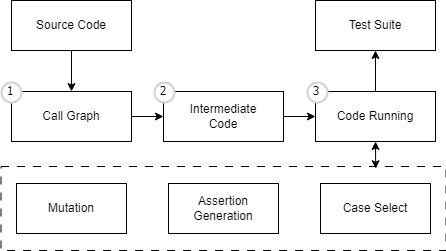
\includegraphics[width=.99\textwidth]{Figures/nxtunit2.png}
  \caption{NxtUnit structure}\label{fig:nxt}
\end{figure}

Having EvoSuite, Randoop and Pynguin as precedents, in 2023 developers from ByteDance (technology Chinese company) presented NxtUnit~\cite{DBLP:conf/ease/WangMCGSP23}, an automatic randomized test generation tool for the programming language Go.
Similar to other state-of-the-art tools, the structure of NxtUnit (see Figure~\ref{fig:nxt}) is composed by an initial source code as input, that is translated into Static Single Assignment form as a way to get a graph with call dependencies between functions.
After this preprocessing, NxtUnit proceeds to synthesize from the call graph a code template that will be filled with appropriate randomly generated parameters and ran during the tool's execution.
All the information for the template synthesis and posterior parameter changes will be done thanks to the information provided by Go Reflect\footnote{https://pkg.go.dev/reflect}.
During the code running phase, NxtUnit focuses in three main tasks: mutation of the parameter inputs at runtime, assertion generation for future regression testing, and test case selection based on code coverage.
Once the tool comes to a halt, the best test cases are exported into a test suite.
In the experiment proposed by the authors, NxtUnit was executed on 500 private ByteDance repositories and 13 out of the 100 highly-rated public repositories of Go, both sets that already contain tests.
The main objective of this setup, was to review the code coverage increase while adding NxtUnit tests to the already existing ones, and it produced an average increase of \(5.51\%\) for the public repositories and \(17.26\%\) for the private ones.

\section{JSEFT}

As an example for automatic test generation in dynamic languages others than Python, JSEFT is presented in 2015 by Mirshokraie et al.~\cite{DBLP:conf/icst/Mirshokraie0P15} as a tool for generating not only unit tests, but also event-driven tests for web applications written in JavaScript.
The general structure of JSEFT is presented in Figure~\ref{fig:jseft} and is composed of three main steps that process the data given by the HTML Document Object Model (DOM):
\begin{itemize}
  \item In (1) the web app is dynamically analysed in order to get all the possible states of the program and, in consequence, construct a state flow graph (SFG)
  \item Then, in step (2), event sequences are extracted from the SFG for the creation of event-driven tests, which will be run in the instrumentalized version of the web app.
  With these executions, JSEFT tries to discover DOM states and entry and exit state points for the creation of function-level unit tests
  \item Finally, the third step (3) mutates the web app at code and DOM level, so functional oracles can be created from the difference between the two states of the original and mutated tests versions
\end{itemize}

\begin{figure}[tb]
  \centering 
  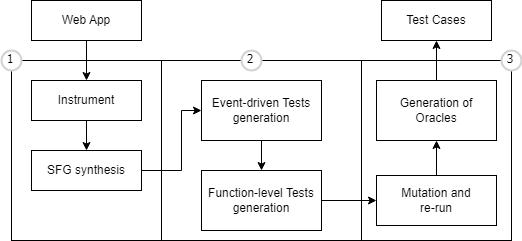
\includegraphics[width=.99\textwidth]{Figures/jseft2.png}
  \caption{JSEFT structure}\label{fig:jseft}
\end{figure}

For the export of event-driven and function-level tests, the frameworks Selenium\footnote{https://www.selenium.dev} and QUnit\footnote{https://qunitjs.com} are used respectively.

The experiment section of the author's paper, shows the study of JSEFT's usage on 13 JavaScript web applications so the line coverage and usefulness of the assertions at the time of finding regression faults.
For the specified metrics, the tool got a \(68.4\%\) of line coverage and a \(100\%\) precision in fault detection.

\section{CodaMOSA}

One of the many tools presented in papers that have cited Pynguin in their research is CodaMOSA~\cite{DBLP:conf/icse/LemieuxILS23}, software created by Microsoft developers, has Pynguin as a base and extends its functionality calling OpenAI's Codex\footnote{https://openai.com/blog/openai-codex} API to get template suggestions for test cases that are in a coverage stall, similar to what this thesis works over.
For the development, the authors used only MOSA as the search algorithm because is the only one that allowed the usage of both line and branch coverage as fitness functions, on the version of Pynguin at the time (0.19.0).

The procedure done by CodaMOSA, queries prompts to Codex after the coverage has not changed in a certain amount of iterations, and from a set of target generations of chromosomes that it statistically chooses to generate a test from either a function, method or constructor.
After that, it deserializes the returned test case from Codex into the internal representation of Pynguin, while applying different heuristics, such as removing nested expressions and use single assignment.

For the benchmark, modules from 35 projects from the Pynguin paper were filtered so just those that do not fail to produce result and those that do not reach \(100\%\) coverage in less than a minute are experimented over.
The baselines for the experimental phase were Pynguin with MOSA and CodexOnly, which while being compared to CodaMOSA were statistically compared using the Mann-Whitney U-Test.
The results showed that CodaMOSA performs significantly better, reaching a higher coverage on 173 more modules compared to MOSA and 279 more modules compared to CodexOnly.

\section{PBT-GPT}

Property-based testing (PBT) is a kind of fuzz testing whose idea is to generate a large amount of random inputs to statistically test a program by checking if the outputs are close to a desired property.
Within this scope, PBT-GPT~\cite{DBLP:journals/corr/abs-2307-04346} is presented by Vikram et al.\ as an implementation of automatic property-based test generation for Python by means of Large Language Model prompting, through Chat-GPT4.
The general idea of this testing approach, is to operate with three different prompting approaches to generate Python tests of specific module methods while using Hypothesis\footnote{https://hypothesis.readthedocs.io/en/latest/}, a PBT library specialized in input generators, and the API documentation of the so-called method.
These three strategies for prompt calling are named and described as the following:

\begin{itemize}
  \item Independently, where both the prompts for the input generator and properties assertion are synthesized from independent instances of Chat-GPT, and then combined in a single Python code snippet
  \item Consecutively, where the prompts are executed sequentially on the same instance of the LLM and combined at the end
  \item Together, where all necessary prompts are combined, and called singularly in an instance of LLM.\@
\end{itemize}

These have as context for the prompt, the LLM being an expert in Python, the LLM needing to review the API documentation, instruction to generate a PBT component, and the desired output format.

For the result evaluation quality, the authors were guided by; generator validity and diversity, that measure either the correct behaviour or diversity of inputs; and property validity, soundness and strength, that measure the encounter of runtime errors, the existence of input/output pairs that violates the property but is valid at the same time, or the ability to check core logic of an API method.
With these guidelines, the modules/methods under test got measurements close to \(100\%\) in generator validity and property validity, and between \(68\%\) and \(88\%\) for the rest of them, which helps conclude that PBT-GPT is a promising starting point to iterate from.

\section{CodeT}

Following the examples of software artefacts presented by Microsoft developers, in 2022 is published a paper regarding CodeT~\cite{DBLP:journals/corr/abs-2207-10397}, a LLM based code generation tool.
The main purpose of CodeT is the solution of a programming problem by generating a code snippet, based on a context containing natural language.
Regardless of this not being in the same direction of the previous software examples, test generation using the same LLM is part of the whole process, although all of these just have the form of a single assertion, together with a set of inputs and the desired output.

\begin{figure}[tb]
  \centering 
  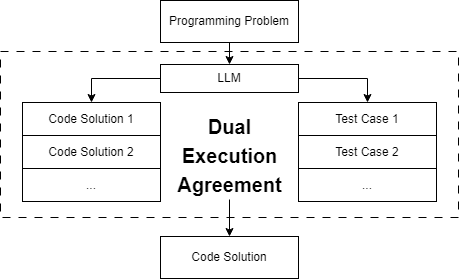
\includegraphics[width=.99\textwidth]{Figures/codet.png}
  \caption{CodeT structure}\label{fig:codet}
\end{figure}

A general structure of CodeT is shown in Figure~\ref{fig:codet}, which also depicts the functioning of it by first, prompting the generation of a set of tests (right on the figure) based on the natural language context of the programming problem, that will later be at the same time the context for the prompting of a set of code snippets (left on the figure).
After the execution of the LLM model is finished and all the outputs are gathered, a Dual execution agreement criterion, based on the RANSAC~\cite{DBLP:journals/cacm/FischlerB81} algorithm, is used to select the best code solution.
The selection in this criterion, is done by forming consensus sets of both code solutions and test cases, by selection a valid pair \((x_\text{code}, y_\text{test})\) as a hypothetical inlier, and grouping it with all tests that are also passed by \(x_\text{code}\) in set \(S_y\) and all other code snippets that pass the same tests as \(x_\text{code}\) in set \(S_x\).
Finally, when all consensus sets \(S_x\) and \(S_y\) are formed from the different valid pairs \((x_\text{code}, y_\text{test})\), those with the highest cardinality \(f(S) = |S_x||S_y|\) will have the best score for selection.

As stated before, CodeT centres around code generation rather than test case generations, which makes the research of this paper focus mainly on metrics such as pass1 or pass100 (correct rate of single solutions, or at least one for every hundred).
Nonetheless, to check the quality of the generated solutions, the authors also covered in their result analysis the code and branch coverage of the snippets generated from the different LLM models.
Almost all the models obtained an overall average coverage of \(95\%\).

\section{MutAP}

Mutation testing is one software testing technique, that aims to measure the ability of a test to reveal bugs.
Taking this approach in mind, Dakhel et al.\@ presented in 2023 MutAP~\cite{DBLP:journals/corr/abs-2308-16557}, another LLM based code generation tool that also introduces prompt augmentation for killing mutants in an iterative process before the actual synthesis of test cases.

\begin{figure}[tb]
  \centering 
  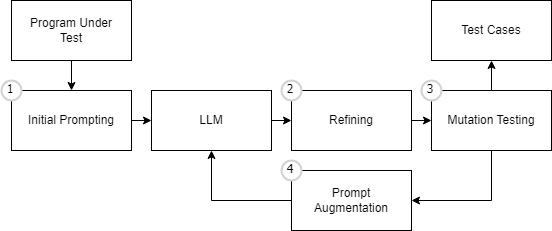
\includegraphics[width=.99\textwidth]{Figures/mutap.png}
  \caption{MutAP structure}\label{fig:mutap}
\end{figure}

A summary of MutAP's structure is shown in Figure~\ref{fig:mutap}, and after inputting a Python Program Under Test (PUT), it commences with the building of an initial prompt for the obtaining of an initial test case.
The first step (1), employs one of the two following learning methods; zero-shot, where the PUT is concatenated after the statement  ``Generate test case for the following code''; and few-shot, which concatenates the PUT after a sequence of pairs of a method and its respective unit test.
After the initial test is synthesized, the second step (2) consists of re-prompting it, so possible syntax errors can be corrected and unintended behaviour can be repaired.
Then, the third step (3) introduces mutations into the PUT using MutPy\footnote{https://pypi.org/project/MutPy/0.3.0/} so that the quality and effectiveness of the tests can be assessed.
At this point, the algorithm of MutAP has a conditional path depending on the number of surviving mutants; if there are none, the test cases are considered finished and generated; and in the contrary case, the prompt augmentation step is followed.
This post conditional step (4), adds information to a new prompt of the LLM, such as the already refined initial test, the statement ``The test function, \(\text{test}()\), cannot detect the fault in the
following code'', one of the mutant survivors, and a final statement ``Provide a new test case to detect the fault in prior code''.

In the experimental trial of this tool's paper, two LLM models were used, OpenAI's Codex and llama2-chat, to be run together with MutAP over the benchmarks; HumanEval, which consists of 164 human written programming problems; and Refactory, consisting of 1710 buggy submissions from students for 5 assignments of a Python programming course.
The overall results mainly cover the mutation score obtained by all the possibles methods of MutAP, obtaining numbers between \(89.13\%\) and \(93.57\%\) on the average over both models and both datasets.

\section{MUTester}

MUTester~\cite{DBLP:journals/corr/abs-2307-00404} is an automatic test generation research software focused on the synthesis of test cases for APIs of the many already existing Deep Learning libraries, i.e. Numpy, Scikit-learn, TensorFlow.
Its structure is presented in Figure~\ref{fig:mutester}, which describes a methodology that solely relies on heuristics regarding the mining of the documentation and knowledge repositories of the APIs in question. 

%TODO: Add numbers

\begin{figure}[tb]
  \centering 
  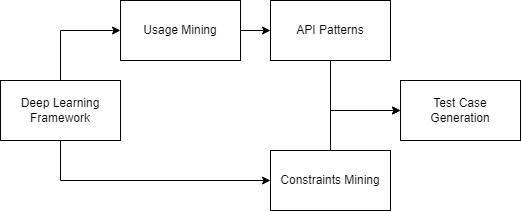
\includegraphics[width=.99\textwidth]{Figures/mutester.png}
  \caption{MUTester structure }\label{fig:mutester}
\end{figure}

The first half of the repository mining (1) is done by applying web scrapping to the documentation pages of different methods of the libraries, so that information regarding input type (via signature definition mining) and constraints can be gathered, which as mentioned before, is crucial for a correct test generation.
Input constraints are collected from the natural language parameter description that is usually presented in Python documentation pages, and rather than extracted using a LLM model, they are identified using by recognizing linguistic patterns.
A last piece of information that is gathered in this step are any code snippet example, so any useful input can be statically analysed.

Stack Overflow is the source of information for the second half of repository mining (2), from where the authors extracted from any related (question, accepted answer) pair the code snippets that had relevant method sequences in them.
Then (3), these method call sequences are studied using the Apriori~algorithm~\cite{agrawal1994fast} to look for intrinsic rules between the calls.

Finally, test case generation (4) is managed as a guided synthesis of a call sequence, that ends in the actual method under test, similar to what Pynguin does, but with the help of all the relationship information obtained in the previous steps.
Similarly, the input generation is conducted.

Throughout the analysis of MUTester, the API documentation and methods of the frameworks,  Scikit-learn, PyTorch, TensorFlow and CNTK were accounted for.
Regarding test coverage, the baselines for the experimentation were Pynguin and a Python implementation of Randoop, which achieved \(34.16\%\) and \(30.87\%\) line coverage in average, versus the results obtained by MUTester, that showed improvements ranging from \(15.72\%\) to \(27\%\).
A Wilcoxon signed-rank
statistical test~\cite{Rey2011} was also applied to the results, obtaining a p-value of less than \(0.05\) suggesting that MUTester outperformed both baselines in the stated datasets.

\section{Differential Prompting}

Detection of software failures can be acknowledged as a benefit that comes from practising software testing.
Following this direction, Li et al.~\cite{li2023nuances} studied the implications of calling ChatGPT with prompts that bypass the insensibility of it to code nuances, so that fail inducing test cases can be generated.
Differential Prompting is the name of the proposed technique, and it divides the failure-inducing generation task in three steps:

\begin{itemize}
  \item Program intention inference, where ChatGPT is asked from a Program Under Test (PUT) to inference and explain the idea of it as a whole
  \item Program generation, where ChatGPT is again prompted to generate code snippets similar to the actual PUT, but by implicitly using the output of the last step as context
  \item Differential testing, in which a test pool of diverse inputs for the PUT is generated in order to test the references from the previous and their outputs.
  In the case that all outputs are consistent with a same set of inputs, this is marked as a ``valid test'' and compared to the output of the PUT.\@
  If they are actually the same and all the branches were already covered, then the program is marked as non-faulty.
  On the contrary, the input set is marked as a failure-inducing test case.
\end{itemize}

With these steps, Differential Prompting was put to the test against Pynguin and an out-of-the-shelf ChatGPT usage to evaluate the benchmarks QuixBugs\footnote{https://github.com/jkoppel/QuixBugs} and Codeforces\footnote{https://codeforces.com} in terms of bug presence.
In these, the success rate of Differential Prompting was \(75\%\) and \(66.7\%\) respectively, in some cases 10 times better than the baselines.

\section{Other applications of automatic test generation}

Rather than only focusing on the application of software testing as a way to get either a good coverage metric or to find defects throughout the development of software, it is possible to make good usage of test case synthesis for other objectives.

A first example is Neatest~\cite{DBLP:conf/kbse/Feldmeier022}, the test generator presented by Feldemeier et al.\@ which is based in neuroevolution and the NEAT algorithm~\cite{stanley2002evolving} for the testing of non-trivial games made on Scratch\footnote{https://scratch.mit.edu}, the educational programming language.

Also, PyLC~\cite{DBLP:conf/sac/SalariEAS23} was presented in 2023 by Ebrahimi et al.\@ as a way of translating Programmable Logic Controller (PLC) representation languages (in graphical or textual form) into Python, to then generate automatic test cases using Pynguin and check the validity of the original systems.

\chapter{Conclusions and Future Work}

\backmatter{}

\printbibliography{}

\end{document}
